\documentclass[12pt]{report}

\usepackage[utf8]{inputenc}
\usepackage[francais]{babel}
\usepackage{graphicx}


\title{Rapport - Projet technologique - Hashiwokakero}
\author{Groupe TM2H}

\begin{document}

\maketitle

\begin{abstract}
Ceci est le résumé du rapport.
\end{abstract}

\tableofcontents

\chapter{Implantation de la librarie hashi}

\section{Création des fonctions de base}

\subsection{Les fonctions de node.c}
\textnormal{Après avoir compris le principe de base d'une partie hashiwokakero, il a était trés facile de définir un \textbf{node} il est composé de ses coordonnées et de son degré.les fonctions de node.c sont relativement simple puisqu'elles sont simplement là pour créer, accéder et supprimer la structure node défini de cette manière:}
\begin{verbatim}
typedef struct node_s {
	int x;
	int y;
	int required_degree;
} *node;
\end{verbatim}

\textnormal{Nous n'avons pas eu de difficulter a réaliser cette partie surtout que le fichier qui nous était donné comme guide (node.h) contenait toutes les informations pour réaliser les fonctions. Le plus dur dans la création des fonctions de base ce trouve dans le game.c}
\subsection{Les fonctions de game.c}
\textnormal{En effet, les fonctions composant game.c ont était un peu plus dur à réaliser. Tout d'abord il a fallut définir la structure game qui contient les noeuds de la partie, le nombre de noeud et les ponts.\\ Pour les noeuds rien de bien compliqué il suffit de créer un tableau de noeud et de donner a la structure le pointeur sur le première élément. Pour les ponts il a fallut un peu plus réfléchir mais nous avons finir par créer un matrice de la taille du nombre de noeud par le nombre de direction (c'est à dire 4). Voilà à quoi ressemble donc notre structure game:}
\begin{verbatim}
typedef struct game_s {
  int nb_nodes;
  node *nodes; 
  int **bridges;
} *game;
\end{verbatim}

\textnormal{Une fois la structure correctement défini il a fallut réaliser les fonctions de création et de destruction d'une partie. Après quelques tests avec valgrind tout semblait coorect.\\ Nous nous sommes donc attaqué au gros du sujet:les fonctions qui font vivre ces structure game et node (l'ajout de pont, la supression de pont, le test de fin de partie...). Au fur et à mesure de notre avancement les tests nous ont permis de décellé de nombreux bug et nous éviter de nombreuses heures de débuggage même si gdb et valgrind nous ont énormément servi durant cette période.\\ Les fonctions les plus complexe, qui nous ont demandé beaucoup de temps sont: can\_add\_bridge\_dir et game\_over.}

\subsubsection{La fonction can\_add\_bridge\_dir}
\textnormal{Cette fonction est une des plus utile du jeu elle permet de savoir si il est possible ou non d'ajouter un pont. Il faut donc vérifier qu'il y est un noeud dans la direction et que le pont ne croise pas un autre pont déjà existant. Pour la première vérification c'est assez simple puisque nous disposons déjà d'une fonction qui fait ça. Pour la deuxième vérification, après avoir chercher un bon moment nous avons choisi de représenter nos ponts sous forme de vecteur et de vérifier par le calcul vectoriel si notre pont croise un autre pont. \\ Supposons que le vecteur AB est notre pont et le vecteur CD l'autre pont alors si vectoriel (vecteur (AB),vecteur (CD))!=0 alors les deux vecteurs se croisent mais il faut vérifier si ils se croisent sur le segment CD avec vectoriel (vecteur (AB),vecteur (AD)) * vectoriel (vecteur (AB),vecteur (AC))< 0\\On a donc une fonction qui prend de la place car il faut récupérer toutes les coordonnées des vecteurs mais qui est plutôt simple.}

\subsubsection{La fonction game\_over}

\chapter{Interface terminal}

\chapter{Caprice des profs}

\chapter{Solveur}
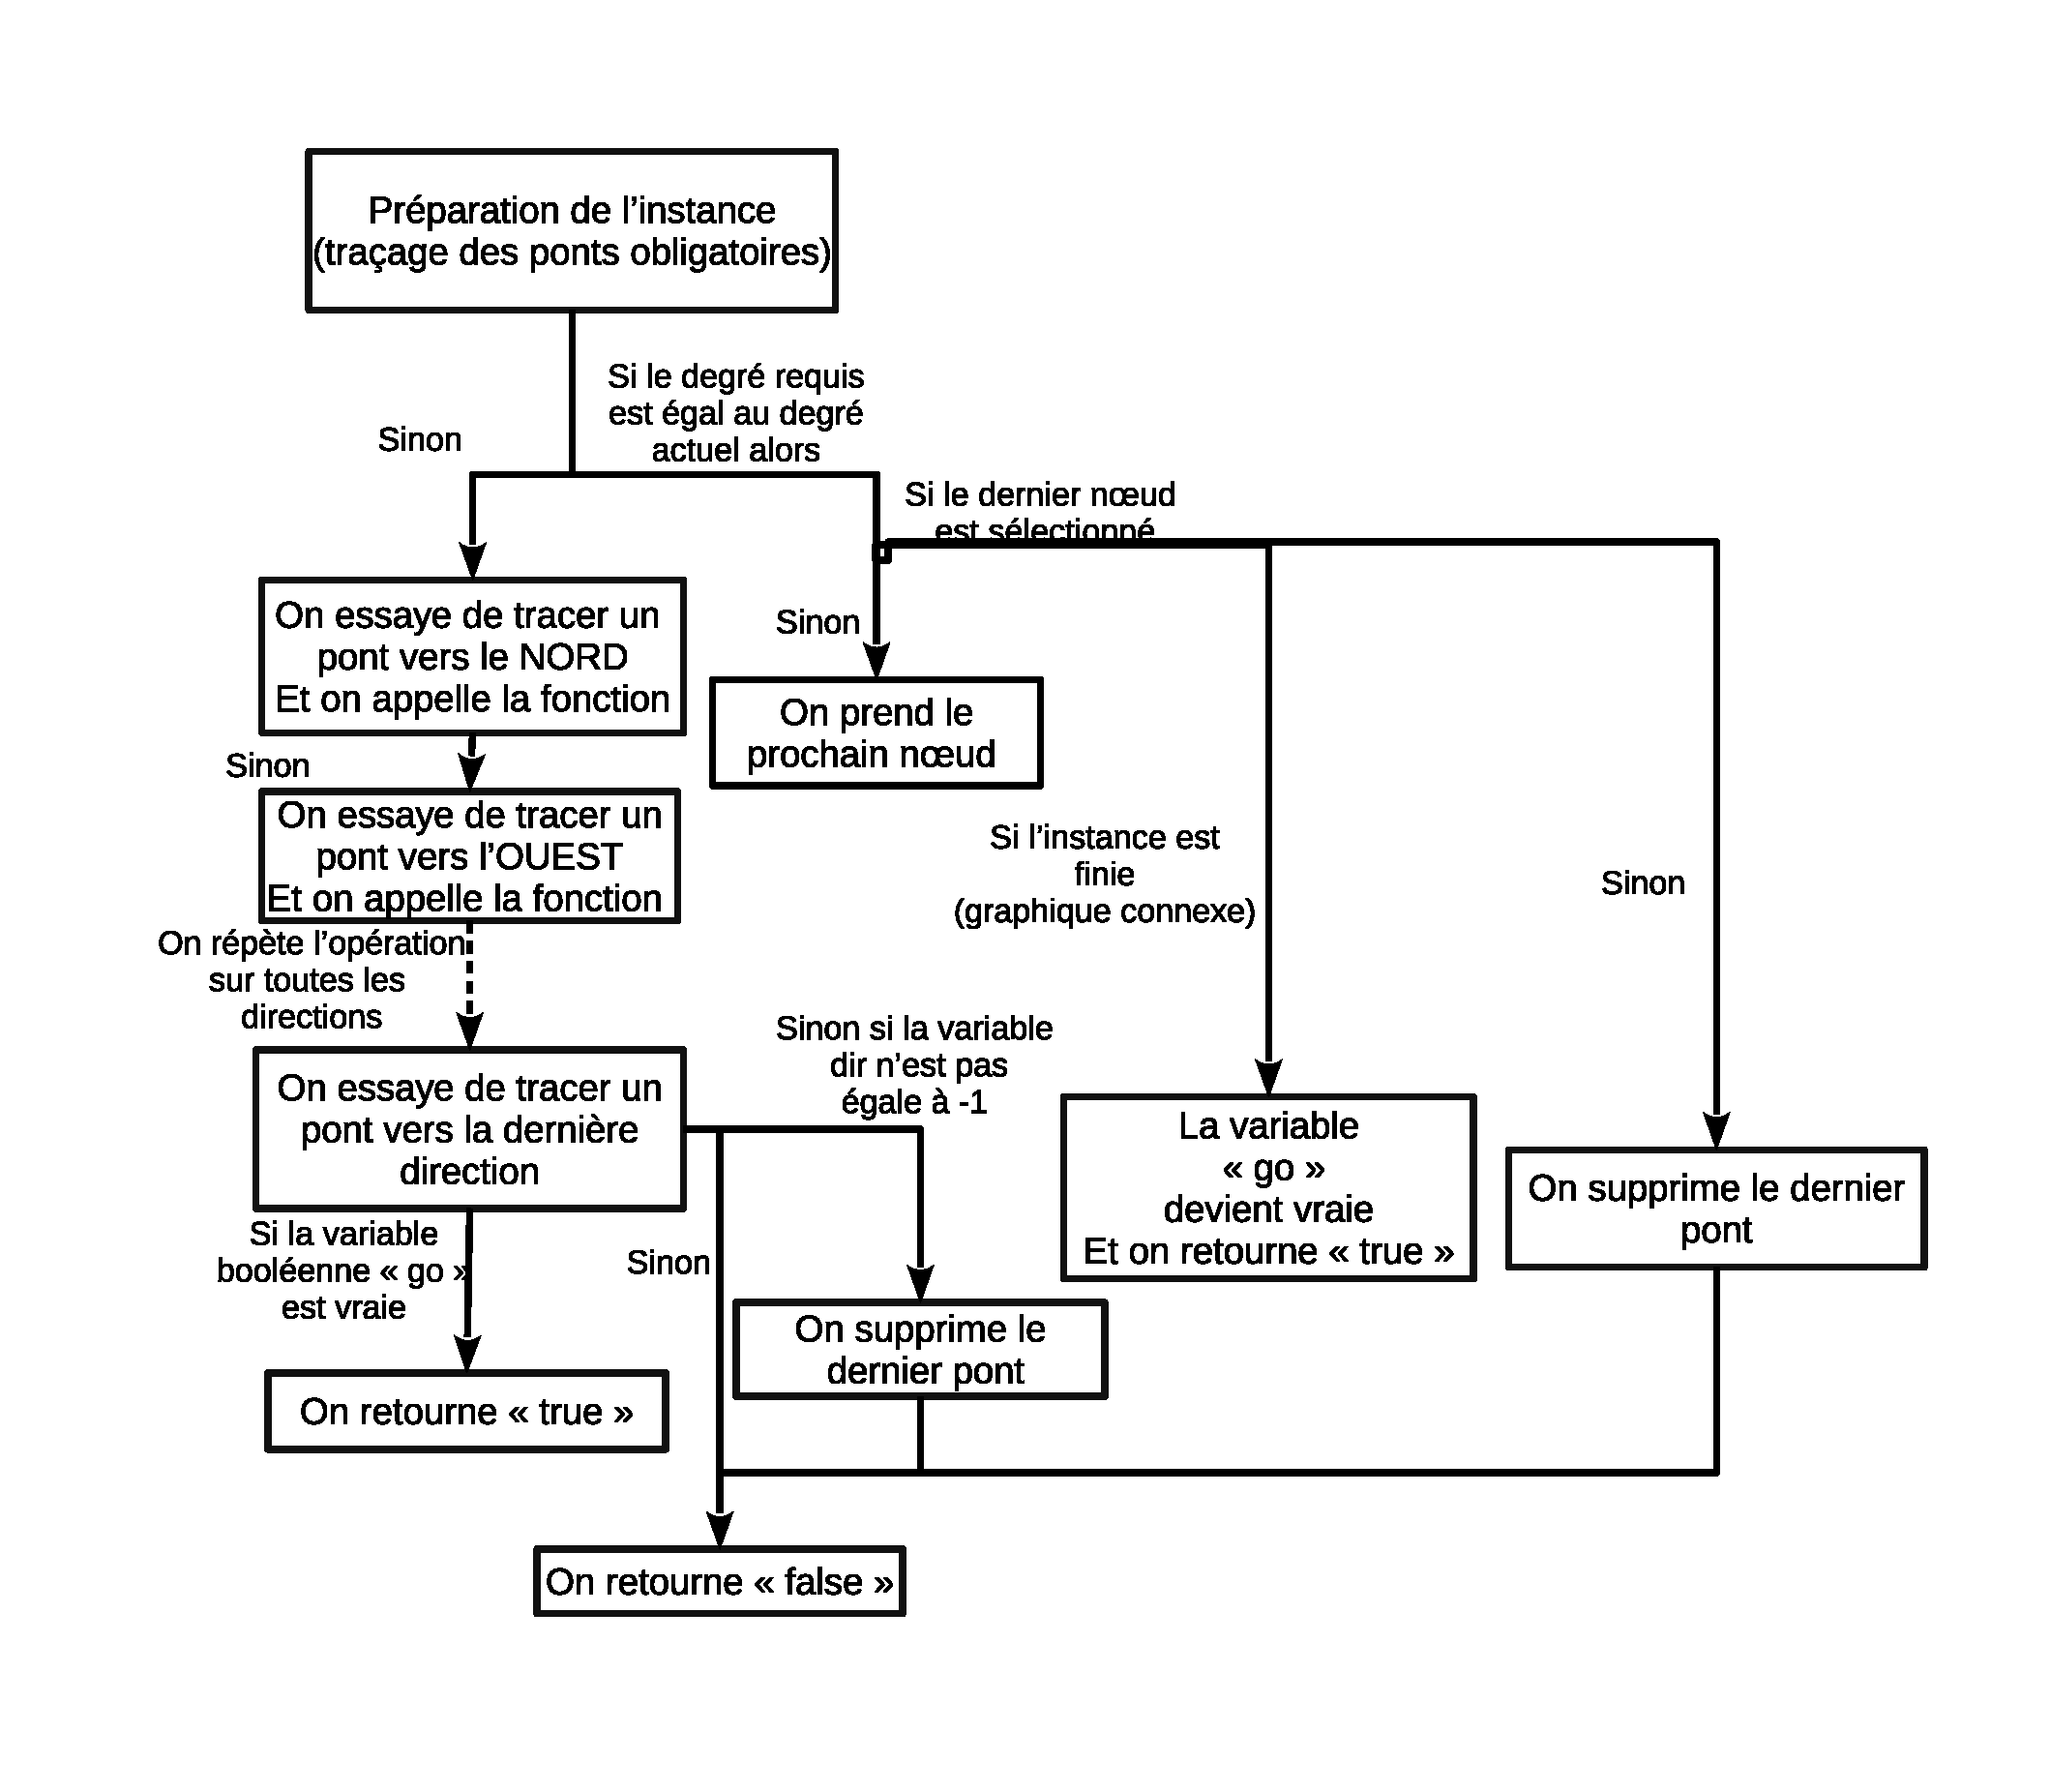
\includegraphics[width = 1.00\textwidth]{explication_solveur.eps}
\section{Explication du graphique}
La préparation de l'instance consiste à tracer les ``ponts obligatoires'',cela concerne les îles qui n'ont qu'une possibilité de liens,
on a déterminé plusieurs cas:
\begin{itemize}
\item Deux îles ne peuvent pas se completer totalement mutuellement, celà formerait un bloc connexe.
\item Si une île a un nombre de ponts possible maximum (en fonction des voisins possiblement atteignable) égale à son degré requis on doit tracer tout ses ponts.
\end{itemize}

Les arguments de la fonction sont:
\begin{itemize}
\item l'instance de jeu (g)
\item le numéro de l'île où nous allons appliquer nos opérations (node\_num)
\item la direction du dernier pont posé utile quand on dépile pour retirer le dernier pont (dir)
\item une variable indiquant si la solution a été trouvée (go)
\end{itemize}

\section{Possibilité d'amélioration}
Pour améliorer ce solveur on pourrait refaire le processus de ``ponts obligatoire'' à chaque fois que l'on fait une action mais celà implique d'avoir une sauvegarde de l'état du jeu pour que lorsque l'on dépile on puisse retirer les ponts posés par ce processus. On a aussi essayé de rajouter une vérification de la possibilité de connexité à chaque fois que l'on pose un pont,comme ça il ne pourrait pas se former de blocs isolés.
\chapter{Interface graphique}
\section{Structure principale de la partie graphique}
La partie graphique est composé de 4 fonctions principale ayant des utilités différentes:
\begin{itemize}
\item Une fonction d'initialisation de l'environnement graphique, qui gère la création des textures, le chargement d'une instance de jeu etc
\item Une fonction de rendu qui s'occupe d'afficher les textures
\item Une fonction qui s'occupe des évenements
\item Une fonction de désallocation qui s'occupe de désallouer les textures et l'instance de jeu
\end{itemize}

\section{Capacités de l'application}
On a réussi à avoir un jeu qui marche avec 4 ou 8 directions et de 2 à 4 ponts, avec d'autres fonctionnalités comme un affichage des ponts possible en passant le pointeur de la souris dessus, des boutons permettant de remettre la partie à 0, de tricher avec le solveur, de charger une partie générée aléatoirement et de sauvegarder.

\chapter{Bonus: Portabilité sur Android}
\end{document}
